\documentclass{article}
\PassOptionsToPackage{hyphens}{url}
\usepackage[hidelinks]{hyperref}
\usepackage{amsmath}
\usepackage{amsthm}
\usepackage{amssymb}
\usepackage{pgfplots}
\usepackage{algpseudocode}
\newcommand{\QED}{\hfill {\qed}}
\newcommand\tab[1][1cm]{\hspace*{#1}}
\usepackage{mathtools}
\DeclarePairedDelimiter\ceil{\lceil}{\rceil}
\DeclarePairedDelimiter\floor{\lfloor}{\rfloor}
\graphicspath{ {./imgs/} }

\title{\#3 Assignment - CMPT 405}
\author{Luiz Fernando Peres de Oliveira - 301288301 - lperesde@sfu.ca}

\begin{document}

\maketitle
\textbf{\#1a)}
\\
Let $G_1$ be a graph with two vertices $A$ and $B$ and an edge $(A, B)$ with weight $1$. For every shortest path tree $T_v$, $v \in V$, $T_v$ is also a MST (it is easy to see, as there is only one tree).
\\
\\
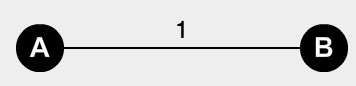
\includegraphics[scale=0.6]{simple_graph_hw3}
\\
\\
\textbf{\#1b)}
\\
Let $G_2$ be a graph with vertices $A, B, C$ and $D$ and edges $(A, B), (A, D), (A,C), (B,C)$ and $(C,D)$, with weights $8, 4, 6, 4 \text{ and } 8$, respectively. Then, no shortest path tree $T_v$ given by Dijkstra's algorithm is a MST.
\\
\\
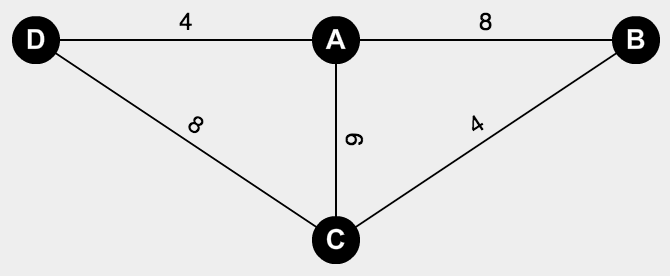
\includegraphics[scale=0.4]{complex_graph_hw3}
\\
\\
MST $= (A,C), (A,D), (B,C)$
\\
$T_a = (A, B), (A, C), (A, D)$
\\
$T_b = (A, B), (A, D), (B, C)$
\\
$T_c = (A, C), (B, C), (C, D)$
\\
$T_d = (A, B), (A, D), (C, D)$
\\
\\
\textbf{\#2)}
\\
\textbf{\#3)}
\\
\textbf{\#4)}
\\
Let $T$ be the unrooted tree decomposition of $G$ and $T'$ be a nice tree decomposition of $T$. The idea of the algorithm is to make any node of $T$ (preferably a internal node with many edges or minimum bag width) its root. So to ease the algorithm, we  preprocess the input $T$: after we root $T$, we go through all the bag leaves $b$ in $T$ and create a new bag for every $v_b \in (b - parent(b))$ and make $b$ their parent. We then run a postorder traversal on $T$ and apply the following rules:
\\
- \textbf{Case 1.} If bag $b$ is a leaf in $T$:
\\
\tab If $b \neq parent(b)$, it must have come from the preprocessing of the original bag $b' - parent(b')$, and therefore $|b| = 1 \leq |parent(b)|$, meaning that we need to add introduce nodes to our nice tree decomposition $T'$ by adding some vertices $v_{parent} \in parent(b)$ and stop when they have the same elements, so we can join the bags later; otherwise, if $b$ and $parent(b)$ have the same elements, we are done.
\\
\\
- \textbf{Case 2.} If bag $b$ is an internal node in $T$:
\\
\tab We know that if $b$ is an internal node, then $b$ is a parent of at least one bag $b'$.  Then, the first step is to add a join node in $T'$ for $b$ and every $b'$, where $parent(b') = b$. Also, because $b$ is an internal node, $b$ has a parent. We need first to get rid of all nodes in $b$ that are not elements of $parent(b)$ (by adding forget nodes to $T'$) and finally add some vertices  $v_{parent} \in parent(b)$ and stop when $b$ and $parent(b)$ have the same elements, so we can join the bags later (by adding introduce nodes to $T'$).
\\
\\
- \textbf{Case 3.} If bag $b$ is the root in $T$:
\\
\tab Finally, if $b$ is the root, we only need to create a join node of all bags $children(b)$ in our final nice tree decomposition $T'$.
\\
\\
The algorithm runs in $O(nk)$ (as per the pseudocode and demonstration below)
\\
\\
Algorithm:\\
\textbf{Input:} \textit{T}
\begin{algorithmic}
\State Make any internal bag (or the bag with minimum width) of $T$ its root.
\For{\textbf{each} bag $b \in T, children(b) = \emptyset $} \textit{// all leaves}
  \State $free_{vs} \gets b - parent(b)$
  \For{\textbf{each} $v \in free_{vs}$}
    \State $T \gets T \cup \{v \}$ such that $parent(v) = b$
  \EndFor
\EndFor
\State $T' \gets \emptyset $
\For{\textbf{each} bag $b \in T_{postorder}$}
  \State $b_{aux} \gets b$
  \If{$children(b) = \emptyset$} \textit{// if leaf}
    \State $T' \gets T' \cup b_{aux}$ \textit{// add leaf node}
    \While{$b_{aux} \neq parent(b)$ }
      \State add introduce node $b_{aux} \cup \{ v_{parent}\} $ in $T'$, for any $ v_{parent} \in parent(b)$,
      \State such that $b_{aux} \cup \{ v_{parent}\} = parent(b_{aux})$
    \EndWhile
  \Else
    \State Create join node in $T'$
    \If{$parent(b) \neq \emptyset$} \textit{// if not root}
      \While{$\exists v \in b \text{, such that } v \notin parent(b)$}
      \State add forget node $b_{aux} - \{ v\} $ in $T'$, for any $ v \notin parent(b)$,
      \State such that $b_{aux} - \{ v\} = parent(b_{aux})$
      \EndWhile
      \While{$b_{aux} \neq parent(b)$ }
      \State add introduce node $b_{aux} \cup \{ v_{parent}\} $ in $T'$,
      \State for any $ v_{parent} \in parent(b)$, such that $b_{aux} \cup \{ v_{parent}\} = parent(b_{aux})$
    \EndWhile
    \EndIf
  \EndIf
\State
\EndFor
\State \textbf{return} $T'$
\end{algorithmic} 
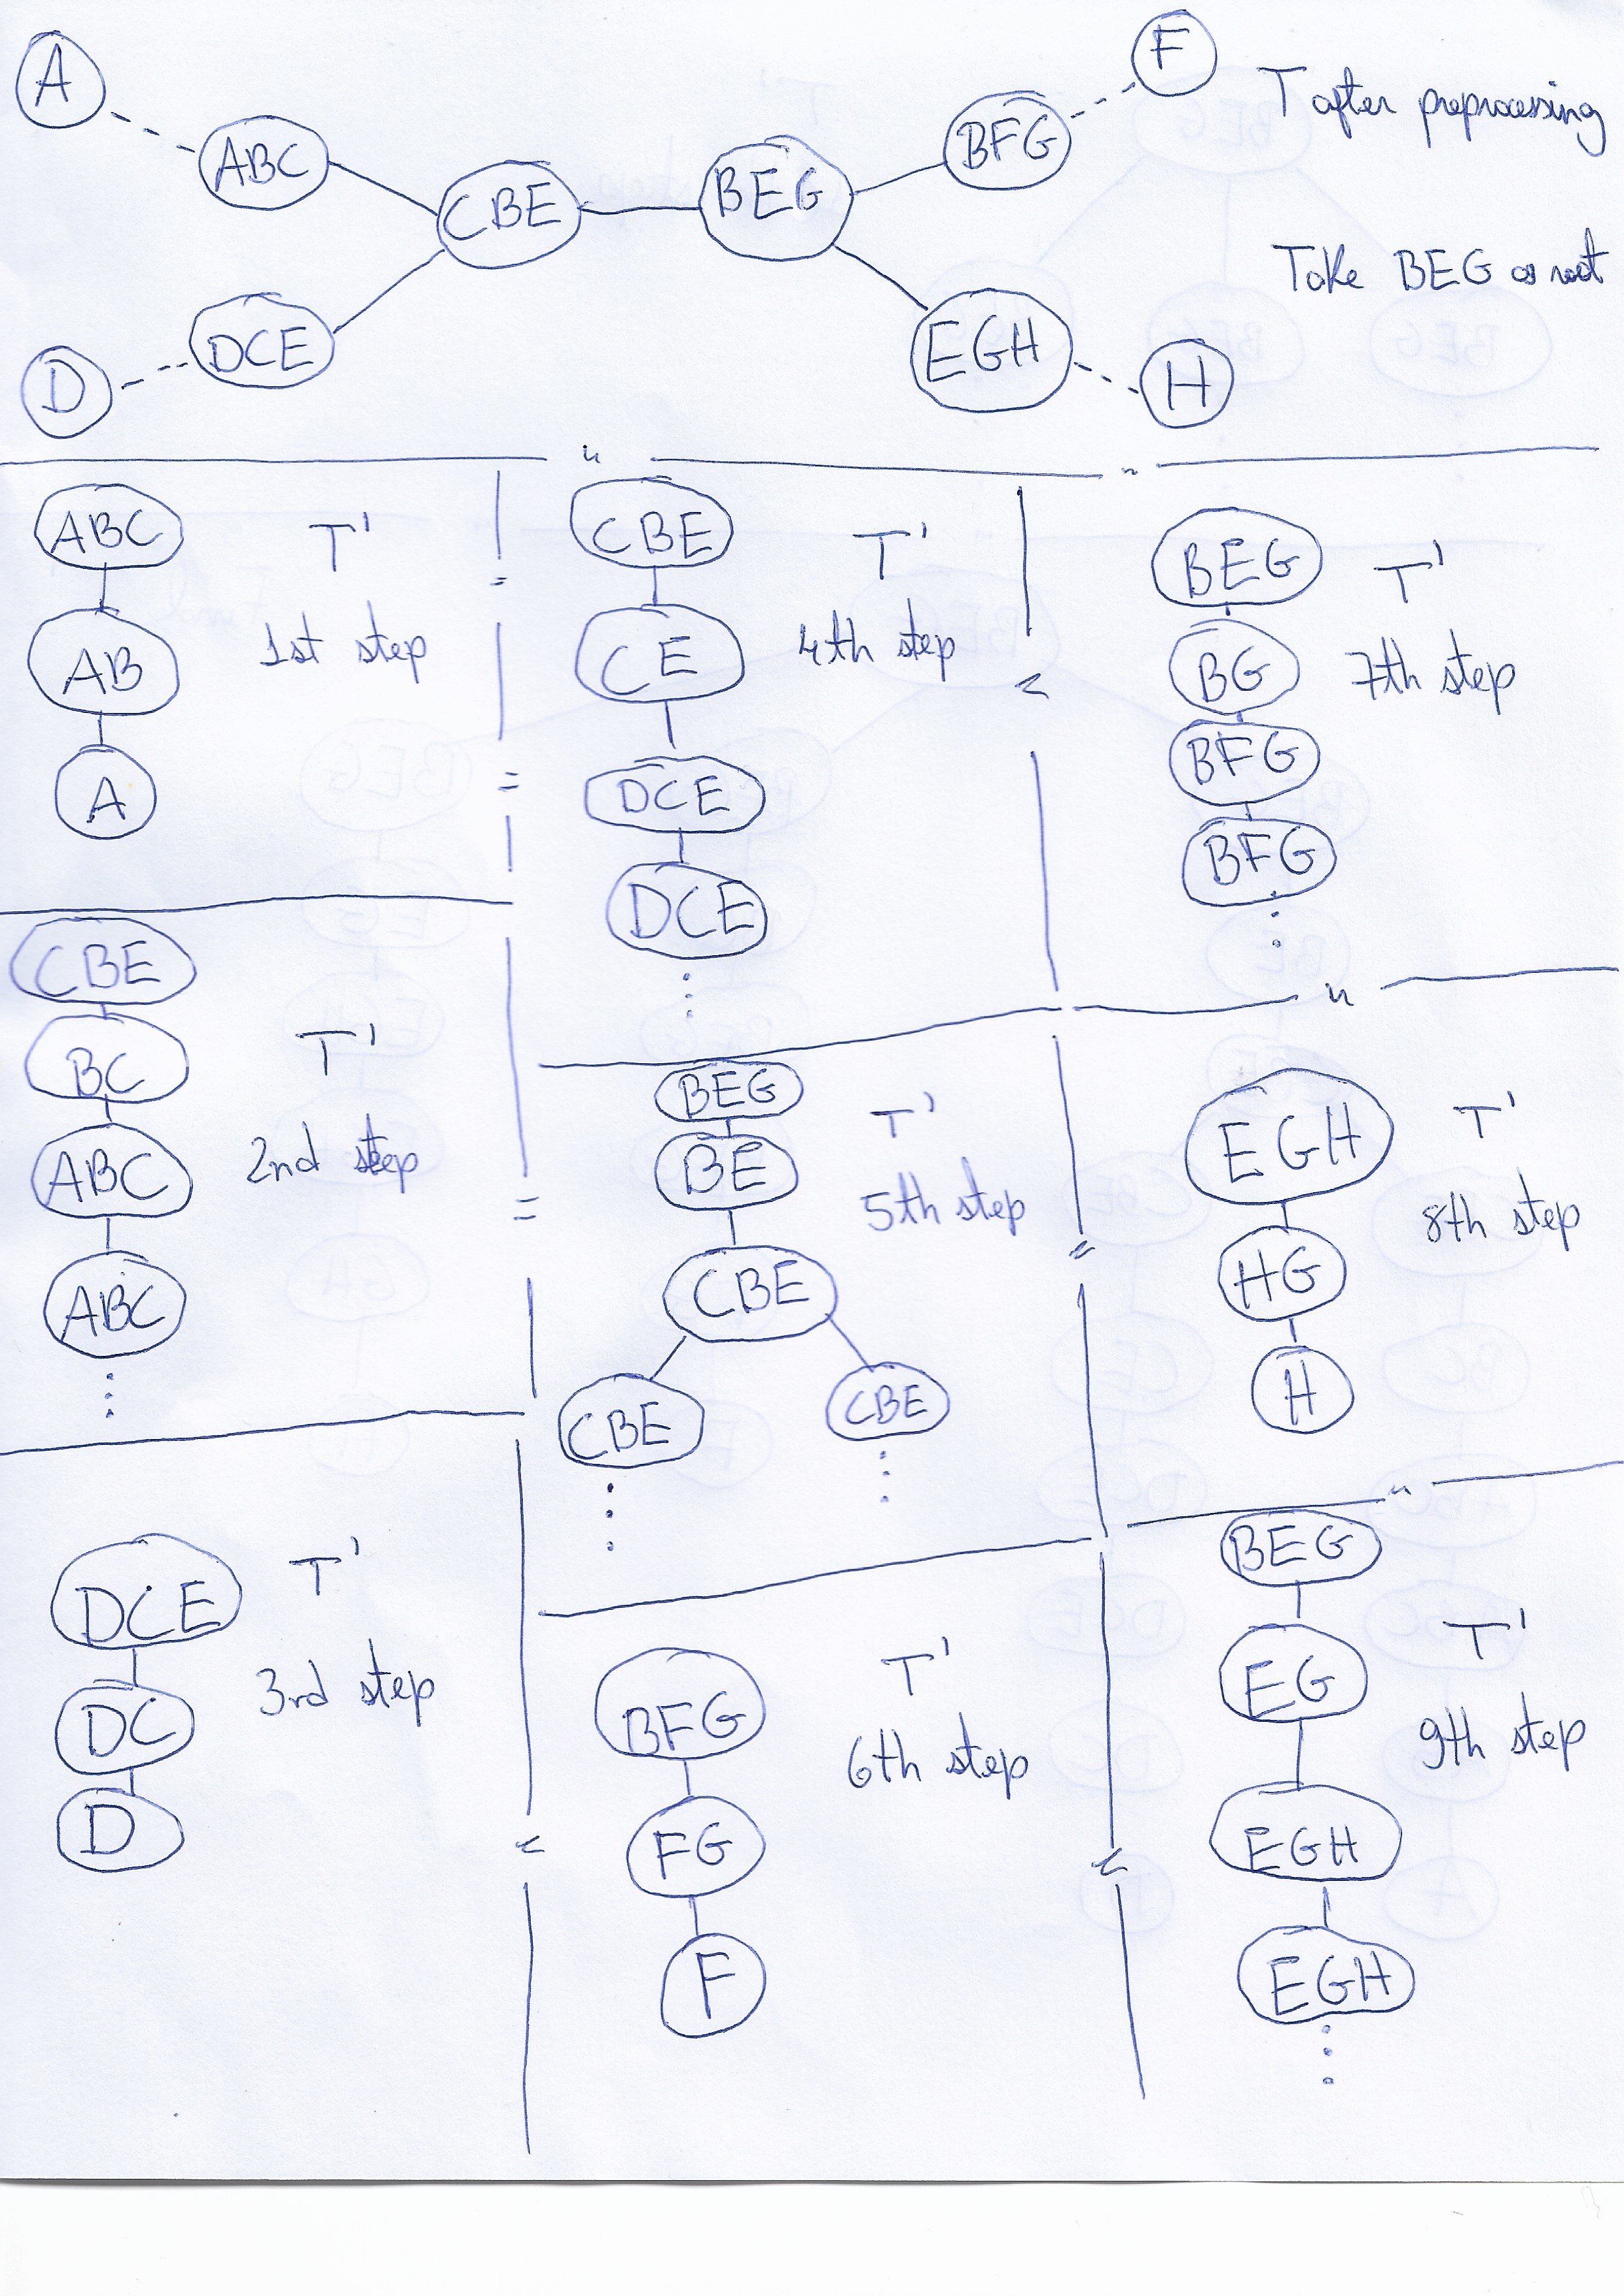
\includegraphics[scale=0.7]{1st_demo_graph_hw3}
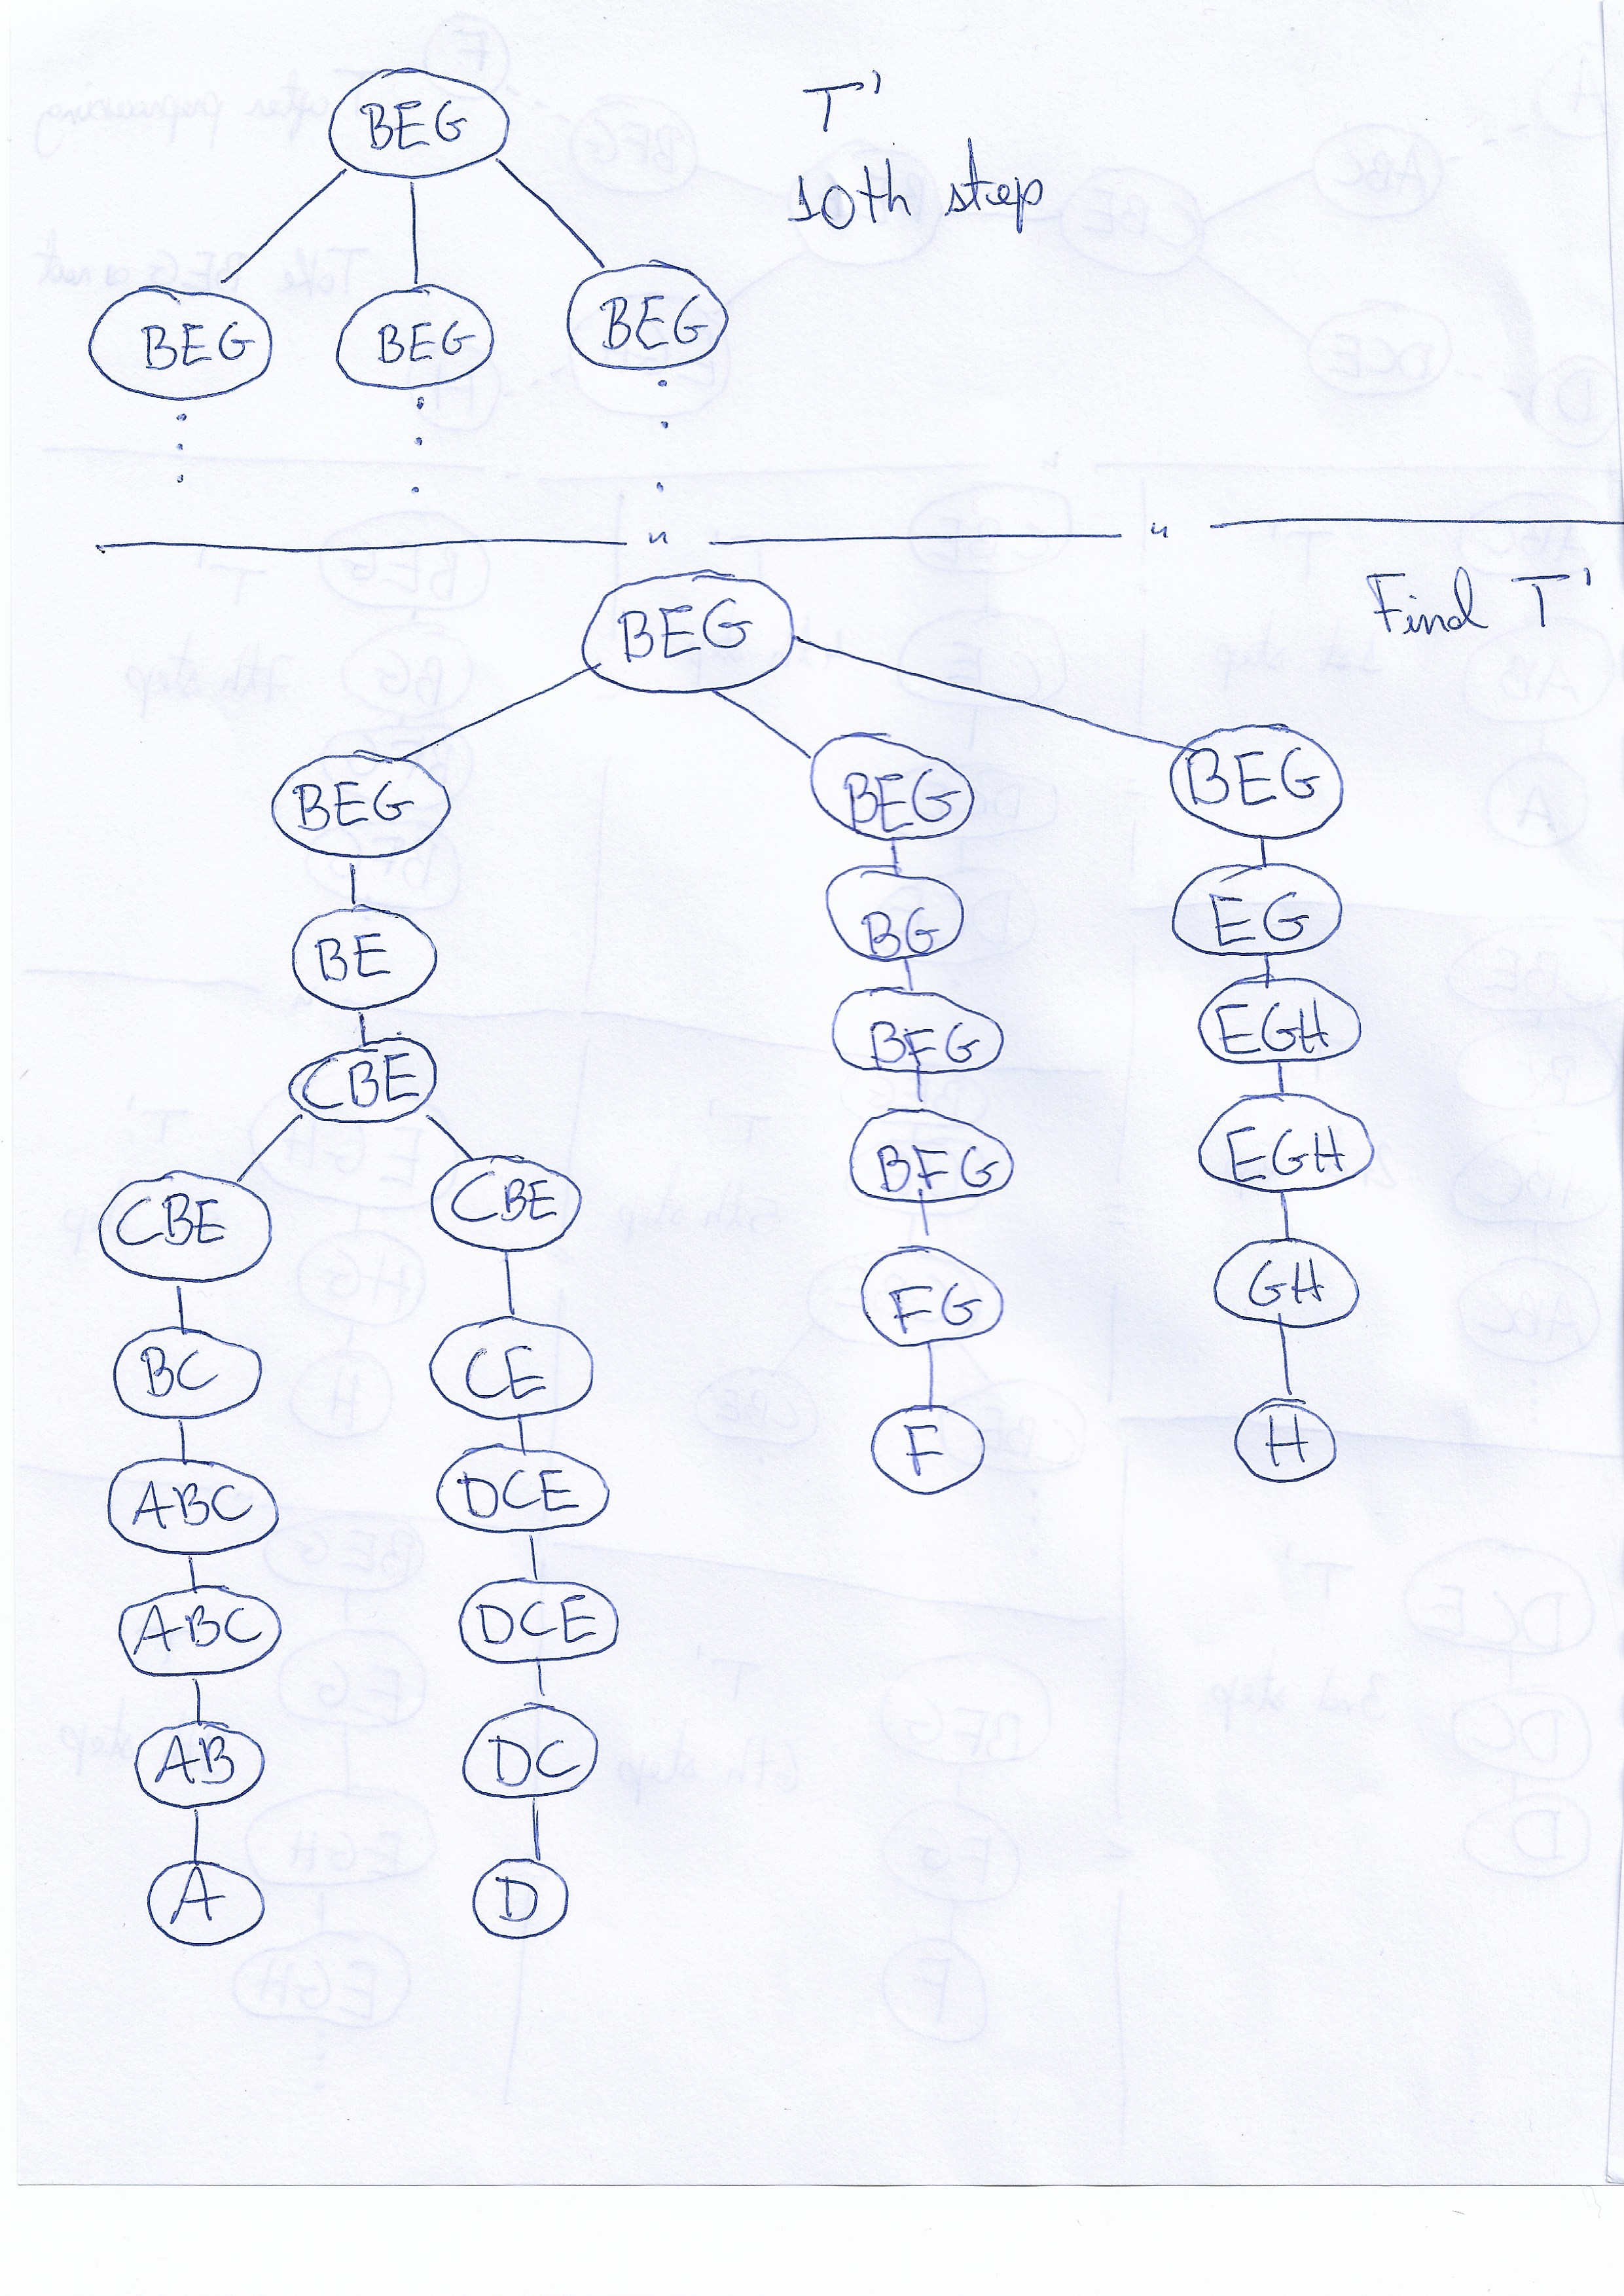
\includegraphics[scale=0.7]{2nd_demo_graph_hw3}
\textbf{\#5)}
\\
\textbf{References}
\\
\end{document}